\section{Aufbau des Versuches}
\label{sec:aufbau}
Ein Foto des Versuchsaufbaus ist in Abbildung \ref{fig:versuchsaufbau} gegeben.
\begin{figure}[H]
  \centering
  \caption{Foto des verwendeten Versuchsaufbaus.}
  \label{fig:versuchsaufbau}
  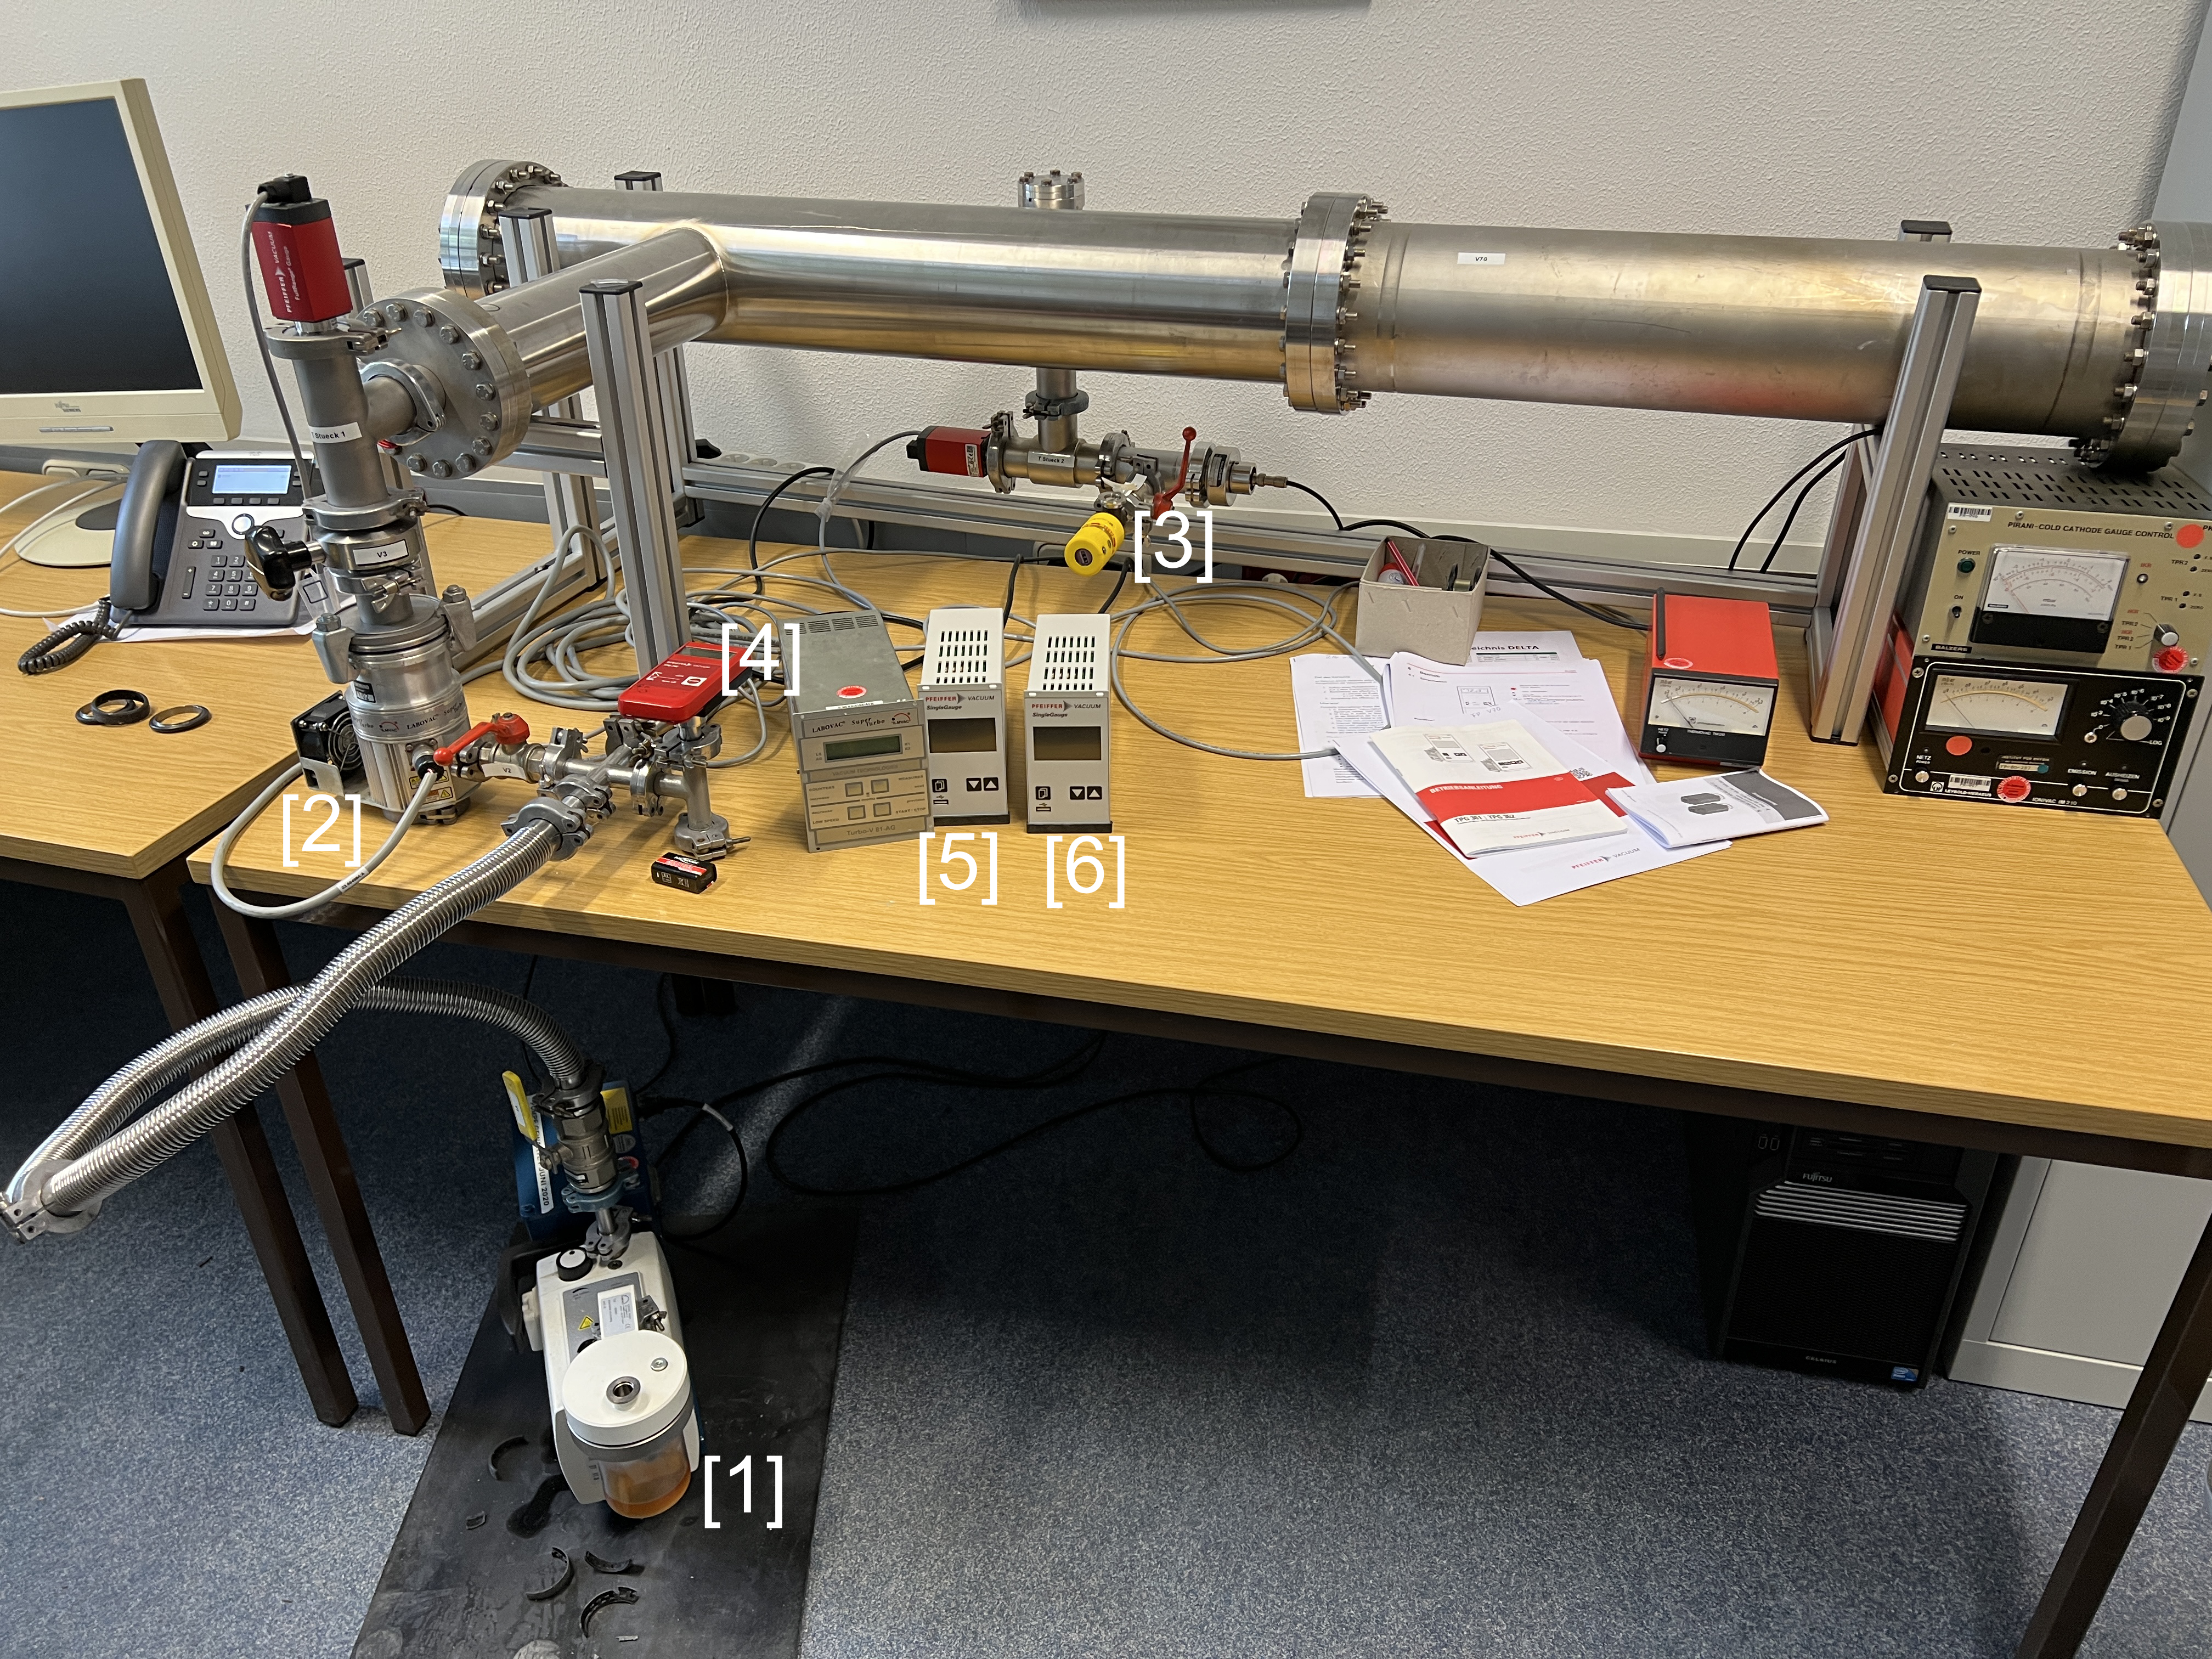
\includegraphics[scale=0.1]{pictures/versuchsaufbau.JPG}
\end{figure}
\noindent
Verwendet wird eine Drehschieberpumpe [1] ILMVAC Typ 300883/AKD16 sowie eine Turbomolekularpumpe [2]
ILMVAC Turbo SST81. Die Pumpen können durch ein Ventil getrennt voneinander betrieben und durch mehrere
Vakuummeter ausgemessen werden.
Bei den verwendeten Vakuummetern handelt es sich um ein kombiniertes
Piezo- und Pirani-Vakuummeter [4] Pfeiffer Vacuum TPG202 sowie zweier kombinierter Pirani- und Kaltkathodenvakuummeter
Pfeiffer Vacuum PKR 360. Das Ventil [3] wird zum Lüften der Apparatur verwendet.

\section{Durchführung des Versuches}
\label{sec:Durchführung}
In diesem Versuch soll eine Evakuierungskurve aufgenommen sowie eine Leckratenmessung
durchgeführt werden. Das genaue Vorgehen wird im Folgenden näher erläutert.

\subsection{Vorbereitung der Messung}
\label{subsec:vorbereitung}
Um die Anlage vor Beginn der Messungen auf Undichtigkeiten zu überprüfen, wird getestet
ob die Drehschieberpumpe nach einem Zeitrahmen von maximal $\SI{10}{\minute}$ einen Enddruck
im Bereich von $\SI{0.03}{\milli\bar}$ erreicht. So wird ein Vorvakuum für die Turbomolekularpumpe
erzeugt, welche nun ebenfalls eingeschaltet wird. Um etwaige Wassereinlagerungen zu entfernen,
kann die Apparatur auch mit einem Heißluftfön ausgeheizt werden. Hiernach sollte mithilfe
der Turbomolekularpumpe ein Enddruck von $\SI{8e-5}{\milli\bar}$ erreicht werden können.
Die erreichten Enddrücke (sowohl für die Drehschieber- als auch für die Turbomolekularpumpe)
werden notiert.

\subsection{Aufnahme der Evakuierungskurven}
\label{subsec:evakkurven}
Für die Aufnahme der Evakuierungskurve der Drehschieberpumpe wird auf den Arbeitsdruckbereich
dieser belüftet. Die Turbomolekularpumpe wird zuvor abgeschaltet. Die Apparatur wird nach
dem Belüften abgedichtet und die Drehschieberpumpe wird eingeschaltet. Der Druckabfall
wird als Funktion der Zeit aufgenommen, indem alle $\SI{10}{\second}$ der Druck notiert wird.
Dies geschieht für eine Messzeit von $\SI{600}{\second}$ und wird dreimal durchgeführt.\\
Für die Aufnahme der Evakuierungskurve der Turbomolekularpumpe wird die Apparatur nicht vollständig
belüftet, da die Turbomolekularpumpe ein Vorvakuuum von mindestens $\SI{0.1}{\milli\bar}$ benötigt.
Daher wird bei laufender Pumpe bis auf
$\SI{5e-3}{\milli\bar}$ belüftet und dann das Ventil geschlossen. Hier wird ebenfalls alle
$\SI{10}{\second}$ der Druck notiert, jedoch nur für eine Messzeit von $\SI{200}{\second}$.
Auch diese Messung wird dreimal wiederholt.

\subsection{Die Leckratenmessung}
\label{subsec:leckratenm}
Um die Leckrate zu ermitteln, wird bei laufender Pumpe und teilweise geöffnetem Nadelventil
ein Gleichgewichtsdruck eingestellt. Dann wird die Pumpe von dem System abgeschoben und der
Druckanstieg als Funktion der Zeit dokumentiert. Dies erfolgt, indem für $\SI{200}{\second}$
(für die Drehschieberpumpe) beziehungsweise $\SI{120}{\second}$ (für die Turbomolekularpumpe)
der Druck alle $\SI{10}{\second}$ (für die Drehschieberpumpe) beziehungsweise alle $\SI{5}{\second}$
(für die Turbomolekularpumpe) notiert wird. Die Messungen für die Drehschieberpumpe und die
Turbomolekularpumpe unterscheiden sich insofern, als dass für die Drehschieberpumpe Gleichgewichtsdrücke
von $\num{0.5}, \num{10}, \num{50}, \SI{100}{\milli\bar}$ eingestellt werden während die
Leckratenmessung für die Turbomolekularpumpe unter Verwendung von den Gleichgewichtsdrücken
$\num{5e-5}, \num{7e-5}, \num{1e-4}, \SI{2e-4}{\milli\bar}$ durchgeführt wird.
